\documentclass[11pt,a4paper]{article}
\usepackage[utf8]{inputenc}
\usepackage[T1]{fontenc}
\usepackage{amsthm} %numéroter les questions
\usepackage[frenchb]{babel}
\usepackage{datetime}
\usepackage{xspace} % typographie IN
\usepackage{hyperref}% hyperliens
\usepackage[all]{hypcap} %lien pointe en haut des figures
\usepackage[french]{varioref} %voir x p y
\usepackage{fancyhdr}% en têtes
%\input cyracc.def
\usepackage[]{graphicx} %include pictures
\usepackage{pgfplots}
\usepackage[]{circuitikz}
\usepackage{ifthen}

\usepackage[top=1.3 in, bottom=1.3 in, left=1.3 in, right=1.3 in]{geometry} % Yeah, that's bad to play with margins
\usepackage[]{pdfpages}

\usepackage[]{attachfile}

\usepackage{float}
\usepackage{subfig}

\usepackage{todonotes} % \missingfigure
\usepackage{gensymb} % \ohm

\usepackage{framed}

\newdateformat{mydate}{2016--2017}%hack pour remplacer \THEYEAR


\newboolean{corrige}
\ifx\correction\undefined
\setboolean{corrige}{false}% pas de corrigé
\else
\setboolean{corrige}{true}%corrigé
\fi

%\setboolean{corrige}{false}% pas de corrigé

\newboolean{annexes}
\setboolean{annexes}{true}%annexes
%\setboolean{annexes}{false}% pas de annexes

\definecolor{darkblue}{rgb}{0,0,0.5}

\newboolean{mos}
%\setboolean{mos}{true}%annexes
\setboolean{mos}{false}% pas de annexes

\usepackage{aeguill} %guillemets

%% fancy header & foot
\pagestyle{fancy}
%Numero du TP :
\def \labonumber {Projet -- Partie 2}
\lhead{[ELEC-H-310] Choucroute numérique\\ \labonumber}
\rhead{\mydate\today\\ page \thepage}
\chead{\ifthenelse{\boolean{corrige}}{Corrigé}{}}
\cfoot{}
%%

\pdfinfo{
/Author (Quentin Delhaye, Ken Hasselmann, ULB -- BEAMS)
/Title (\labonumber ELEC-H-310)
/ModDate (D:\pdfdate)
}

\hypersetup{
pdftitle={\labonumber [ELEC-H-310] Choucroute numérique},
pdfauthor={Quentin Delhaye, Ken Hasselmann, ULB -- BEAMS},
pdfsubject={}
}

\theoremstyle{definition}% questions pas en italique
\newtheorem{Q}{Question}[] % numéroter les questions [section] ou non []

\newcommand{\reponse}[1]{% pour intégrer une réponse : \reponse{texte} : sera inclus si \boolean{corrige}
	\ifthenelse {\boolean{corrige}} {\paragraph{Réponse :} \color{darkblue}   #1\color{black}} {}
 }

\newcommand{\addcontentslinenono}[4]{\addtocontents{#1}{\protect\contentsline{#2}{#3}{#4}{}}}

\date{\vspace{-1.7cm}\mydate\today}
\title{\vspace{-2cm}\labonumber\\ Électronique numérique [ELEC-H-310]\\Conception d'une régulation de refroidissement~: \\ acquisition et contrôle de la température\ifthenelse{\boolean{corrige}}{~\\Corrigé}{}}

%\author{\vspace{-1cm}}%\textsc{Yannick Allard}}

\setlength{\parskip}{0.2cm plus2mm minus1mm} %espacement entre §
\setlength{\parindent}{0pt}


















\begin{document}
\pagestyle{empty}
\maketitle
% \vspace*{-1cm}




% ########   ##     ##  ##########  
% ##     ##  ##     ##      ##      
% ##     ##  ##     ##      ##      
% ########   ##     ##      ##      
% ##     ##  ##     ##      ##      
% ##     ##  ##     ##      ##      
% ########    #######       ##      

\section*{But de la manipulation}
Durant trois laboratoires, vous serez amenés à réaliser une mini-climatisation basée sur un ventilateur à hélice.
Il vous sera également demandé de pouvoir interagir localement (clavier) avec le dispositif.

Dans ce second labo, vous réaliserez le contrôle en boucle fermée de la température d’un élément chauffant.
Vous agirez sur cette température par l’entremise de l’hélice utilisée.


\section*{Prérequis}
Avant d’entrer au laboratoire, il est demandé de lire le cahier des charges du projet «~Conception d’une régulation de refroidissement~».


\section*{Objectifs}
À la fin de ce laboratoire, vous devez être capables~:
\begin{itemize}
	\item De dimensionner une chaîne d'acquisition pour l'utilisation sur $\mu$C.
	\item De réaliser une régulation simple.
\end{itemize}


\newpage




% ########   ##      ##  ##########  ########     #####    
%    ##      ###     ##      ##      ##     ##  ##     ##  
%    ##      ## ##   ##      ##      ##     ##  ##     ##  
%    ##      ##  ##  ##      ##      ########   ##     ##  
%    ##      ##   ## ##      ##      ##   ##    ##     ##  
%    ##      ##     ###      ##      ##    ##   ##     ##  
% ########   ##      ##      ##      ##     ##    #####    


\section{Introduction}
Durant trois laboratoires, vous serez amenés à réaliser une mini-climatisation basée sur un ventilateur à hélice.
Il vous sera également demandé de pouvoir interagir localement (clavier) avec le dispositif.

Lors de ce laboratoire, votre premier but sera de mesurer la température d’un élément chauffant.
Pour ce faire, vous devrez concevoir une chaine d’acquisition permettant d’amplifier une tension représentant la température actuelle.

Sur base de cette mesure, et de la température voulue, vous réaliser un régulateur permettant de s’assurer que la température de la pièce est bien celle de référence.






%    ###      #######     #####    ##     ##  ########    #######   ########   ##########  ########     #####    ##      ##  
%   ## ##    ##     ##  ##     ##  ##     ##     ##      ##     ##     ##          ##         ##      ##     ##  ###     ##  
%  ##   ##   ##         ##     ##  ##     ##     ##      ##            ##          ##         ##      ##     ##  ## ##   ##  
% ##     ##  ##         ##     ##  ##     ##     ##       #######      ##          ##         ##      ##     ##  ##  ##  ##  
% #########  ##         ##    # #  ##     ##     ##             ##     ##          ##         ##      ##     ##  ##   ## ##  
% ##     ##  ##     ##    #### #   ##     ##     ##      ##     ##     ##          ##         ##      ##     ##  ##     ###  
% ##     ##   #######           #   #######   ########    #######   ########       ##      ########     #####    ##      ##  



\section{Conception de la chaîne d'acquisition}
Comme expliqué dans le cahier des charges, la mesure primaire de la température se fait en faisant passer un courant constant et connu à travers une résistance dont la valeur change avec la température.
Cette mesure, de faible amplitude, doit ensuite être amplifiée avant d’être numérisée (voir figure~\ref{fig:acquisition}).

\begin{figure}[H]
\center
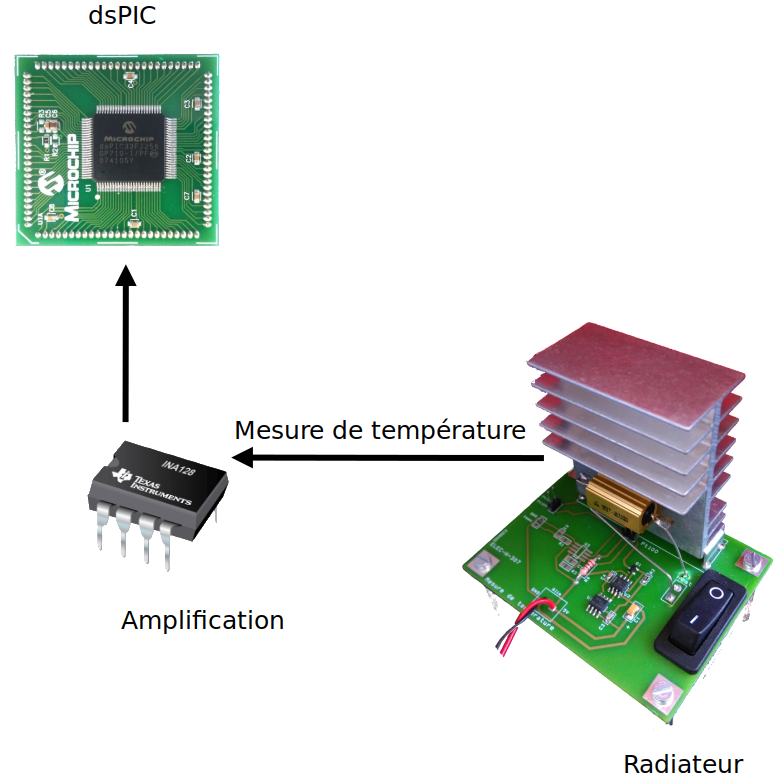
\includegraphics[width=0.8\textwidth]{acquisition}
\caption{Chaîne d'acquisition de la température.}
\label{fig:acquisition}
\end{figure}

\begin{itemize}
	\item Sachant que la température peut atteindre 45$\celsius$, quelle est la tension maximum mesurable aux bornes de la résistance~?
	\item Le convertisseur analogique-numérique numérise la tension sur 10 bits et est alimenté en 3.3V, quelle est dès lors sa résolution~?
\end{itemize}

Nous allons maintenant concevoir la chaîne d'amplification.
\begin{itemize}
	\item Pourquoi est-il nécessaire d’amplifer~?
	\item Pourquoi l’amplification doit-elle être différentielle~?
	\item À l’aide de la notice de l’INA128, dimensionnez la résistance de gain.
	\item Réalisez le montage sur protoboard et vérifiez son fonctionnement.
\end{itemize}






%  #######     #####    ##      ##  #########  ########    #######   ##     ##  ########      ###     ##########  ########     #####    ##      ##  
% ##     ##  ##     ##  ###     ##  ##            ##      ##         ##     ##  ##     ##    ## ##        ##         ##      ##     ##  ###     ##  
% ##         ##     ##  ## ##   ##  ##            ##      ##         ##     ##  ##     ##   ##   ##       ##         ##      ##     ##  ## ##   ##  
% ##         ##     ##  ##  ##  ##  ######        ##      ##   ####  ##     ##  ########   ##     ##      ##         ##      ##     ##  ##  ##  ##  
% ##         ##     ##  ##   ## ##  ##            ##      ##     ##  ##     ##  ##   ##    #########      ##         ##      ##     ##  ##   ## ##  
% ##     ##  ##     ##  ##     ###  ##            ##      ##     ##  ##     ##  ##    ##   ##     ##      ##         ##      ##     ##  ##     ###  
%  #######     #####    ##      ##  ##         ########   ########    #######   ##     ##  ##     ##      ##      ########     #####    ##      ##  



\section{Configuration du convertisseur A/N}
Vous allez maintenant programmer le convertisseur analogique/numérique de sorte à obtenir une image numérique de la température.
\begin{itemize}
	\item À l’aide du guide de programmation, configurez le convertisseur de sorte à numériser la température toutes les 10~ms (attention, des étapes supplémentaires sont nécessaires par rapport au labo 2).
	\item Sur base de votre chaine d’acquisition, écrivez une fonction permettant de retrouver la température en $\celsius$ à partir du nombre sortant du convertisseur.
	\item Écrivez une seconde fonction permettant d’afficher la température sur l’écran LCD, avec une fréquence de rafraichissement d’une seconde.
\end{itemize}






% ########   #########   #######   ##     ##  ##            ###     ##########  ########     #####    ##      ##  
% ##     ##  ##         ##         ##     ##  ##           ## ##        ##         ##      ##     ##  ###     ##  
% ##     ##  ##         ##         ##     ##  ##          ##   ##       ##         ##      ##     ##  ## ##   ##  
% ########   ######     ##   ####  ##     ##  ##         ##     ##      ##         ##      ##     ##  ##  ##  ##  
% ##   ##    ##         ##     ##  ##     ##  ##         #########      ##         ##      ##     ##  ##   ## ##  
% ##    ##   ##         ##     ##  ##     ##  ##         ##     ##      ##         ##      ##     ##  ##     ###  
% ##     ##  #########  ########    #######   #########  ##     ##      ##      ########     #####    ##      ##  



\section{Régulation de la température}
Vous avez maintenant tous les éléments nécessaires pour réaliser le contrôle de la température.
Il ne reste plus qu’à réaliser le régulateur (figure~\ref{fig:regulation}).

\begin{figure}[h]
\center
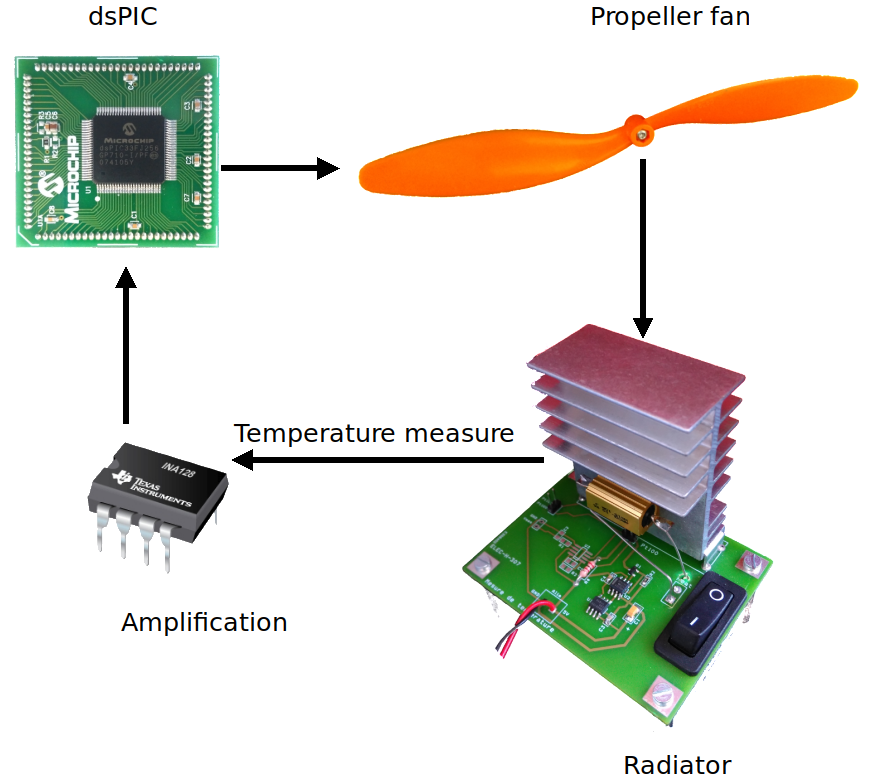
\includegraphics[width=0.8\textwidth]{regulation}
\caption{Boucle de régulation}
\label{fig:regulation}
\end{figure}

\begin{itemize}
	\item Écrivez une fonction prenant comme argument la température de référence et la température actuelle.
	Cette fonction de régulation devra ajuster la vitesse de rotation du ventilateur, de sorte à régler la température.
	Le choix du régulateur est libre, mais il n’est pas utile d’en faire un trop complexe.
	\item Choisissez une température de référence de 28$\celsius$, et vérifiez le bon fonctionnement.
\end{itemize}



\end{document}
